

\chapter{Agents Propagation Model}
\label{ch:Agents Propagation Model}

In this chapter we describe the information propagation process among a group of rational agents taking place in discrete time. We first provide a probabilistic representation of the information shared by this group of individuals under our assumptions followed by the propagation rules of our model. Finally, we conclude this chapter with an analysis of agents news-sharing process dynamics and the structural properties that arise from those. Although this thesis is provides all the basic background, we suggest the reader to study \cite{papanastasiou} which is the basis of our model.


\section{A Probabilistic Representation of News}
\label{sec:FKNews param}
We assume that each event in the world is characterized by a binary state $\Theta \in \{Y,N\}$ \footnote{This model supports events with more than two states but for the sake of simplicity we stay in a binary model.} which is unobservant by a group of individuals (we call them agents) and they are of interest to find the exact value of $\Theta$. Agents may create informative content in forms of news articles (we call them stories) that contain information over the ground truth. These stories are described by $m \in \{y,n\}$ and state the creators realization of the ground truth $\Theta$. Each story can be characterized by another unobservant variable $V \in \{F,T\}$ which declares the validity of its content. If the stance of a story aligns with the actual event, we have $V=T$ with respect to $\Theta$ (truthful story). In the other hand we have $V=F$ with respect to $\Theta$ (fake story) whenever we are dealing with stories that are uninformative or misleading in respect to $\Theta$. \footnote{We should mention that our model does not capture the intention of creating fake stories, i.e. deliberately creating fake information or bad journalism.} 

\begin{table}[t]\
\centering
\captionsetup{justification=centering}
\caption{The probability distribution of truthful stories ($V=T$ left) and fake stories($V=F$ right) with respect to the ground truth.}
\label{tab:Message Type}
\begin{tabular}{ l  l }
\begin{tabular}{| c || c | c |}
\hline
$P(m \mid ( \Theta , V) )$ & $\Theta = Y$ & $\Theta = N$ \\
\hline
\hline
$m=y$                    & $a$          & $1-a$        \\
\hline
$m=n$                    & $1-a$        & $a$         \\
\hline
\end{tabular}
&
\begin{tabular}{| c || c | c |}
\hline
$P(m \mid ( \Theta , V) )$ & $\Theta = Y$ & $\Theta = N$ \\
\hline
\hline
$m=y$                    & $\beta$          & $\beta$        \\
\hline
$m=n$                    & $1-\beta$        & $1-\beta$         \\
\hline
\end{tabular}
\end{tabular}
\end{table}

In table ~\ref{tab:Message Type} we have the probability distributions for both possible types of messages when we are characterizing them with their validity $V$. The signal-generating process for truthful stories is described by the system of equations:

\begin{align}
	\begin{split}
		\mathbb{P} ( y \mid (Y,T)) = \mathbb{P} ( n \mid(N,T)) &=a \\
		\mathbb{P} ( y \mid (N,T)) = \mathbb{P} ( n \mid(Y,T)) &=1-a
	\end{split}
\end{align}


where $a$ can be translated as the persuasiveness of source without any other prior knowledge (i.e. the sharing history) or the probability of a story that shares the same stance as the ground truth thus having truthful validity. We assume that the persuasiveness is $a \in (0.5,1)$ and it is known parameter in our ecosystem. On contrary, when we are dealing with fake stories the signal-generating process is:
\begin{align}
	\begin{split}
		\mathbb{P} ( y \mid (Y,F)) &= \mathbb{P} ( y \mid(N,F)) =\beta \\
		\mathbb{P} ( n \mid (Y,F)) &= \mathbb{P} ( n \mid(N,F)) =1-\beta
	\end{split}
\end{align}
From the above equations we notice that the probabilities of stories $m$ in both cases remain the same over different values of $\Theta$. This reflects the fact that the content of a story is totally uninformative and is randomly aligned with one of the possible states for ground truth, i.e if $\beta > 0.5$ the author of a the story pushes his own agenda with a false narrative described by a story of type $m=y$. Another observable variable, that we assume it is common knowledge, is the percentage of fake stories that circulate in our social infrastructure. Platform can monitor the validity of previous stories and calculate the frequency, or an approximation, of fake stories denoted as $v$. We can also express this quantity as the probability of a newly created story being fake without any prior evidence, $v= \mathbb{P} ( V=F )$. Those parameters conclude all possible outcomes of a message type, in terms of validity and stance, that describes a binary state of an event. In the next section we provide an example in order to illustrate how those parameters work in a real scenario.

\subsection{Example}
\label{subsec:exmpl}

We now provide an illustrative example in order to understand the role of those parameters named in the previous section. There are several real world incidents we can reference from fact checking sites, but we use a fabricated example for the sake of simplicity.~\footnote{Some examples fact checking sites are snopes \url{https://www.snopes.com/} and politifact \url{https://www.politifact.com/}.}

Suppose we have the next claim about COVID-19:

\textit{"University of Ioannina study finds that mortality rate of COVID-19 is lower in countries with warmer climate."}

In our example, we have the ground truth, described by $\Theta \in \{Y,N\}$ where $Y$ aligns with the content of the sentence, in other words $Y$ is interpreted as \textit{"Yes, mortality rate is lower in warmer climates"}, while $N$ presents no link between climate and the mortality rate of COVID-19. The content of the article support $\Theta = Y$ so we have that $m=y$. Also we expect that a claim made by university of Ioannina would be highly persuasive since it would be researched with valid methods so $a$ is expected to be over $85\%$, taken at face value. This means that we are likely to adopt the validity of that claim no matter the content of the research, only by attributing the persuasiveness of the source as an authoritative entity in the research domain. Another case is when we expect from the source of a story to be in interest to push a story that aligns with a narrative. For example, if we knew that university of Ioannina had benefit from supporting $Y$, then it might be the case that it produces a fake story, whose stance $m=y$ holds with probability $\beta$, independently of the actual value of the ground-truth variable $\Theta$. Another scenario is when we expect that the source is not biased but we distrust their journalistic effort or the claim is more likely to be false. Remember that $\beta$ expresses the bias of a source to produce a fake story that supports either $Y$ or $N$, while $\beta = 0.5 $ means that the fake story is produced randomly to align with one side.

Now let's assume that all stories circulating our social structure is probably truthful. This means that $v$ is approaching $0\%$ and in order to simplify things, let $v=0$. An agent with prior belief $\theta = \mathbb{P} (\Theta = Y)$ will update his posterior belief as:
$$\theta_{posterior} =  \mathbb{P} (\Theta = Y \mid m=y ) = \frac{a \theta}{a \theta +(1-a)(1-\theta)}$$
which is greater that his prior belief $\theta$ since $a \in (0.5,1)$. In other words, the fact that all stories are truthful strengthens agent posterior belief that $\Theta = Y$ or equivalent that the story is truthful, $V=T$ and $m=y$. On the contrary, if all the stories shared within the social network are almost certainly fake, $v=1$, we have that:
$$\theta_{posterior} = \frac{\beta \theta}{\beta \theta +(1-\theta)\beta}=\theta_{prior}$$
We see that posterior belief remains the same as our prior opinion since any new information over previous actions would not affect agents  posterior belief. 

\section{Sharing Process and Agents Behavior}
\label{sec:SharingProc}

We assume that a group of infinite rational agents act in a discrete time $t \in \{1,2,...\}$ (we refer time as round $t$) based on various parameters. Each agent is characterized by its own prior belief over ground truth which we assume that is an \textit{iid} draw from a Gaussian distribution. We denote agent $i$'s prior belief as $\theta_{i0} := \mathbb{P} ( \Theta = Y ) $. \footnote{Without loss of generality, we assume that prior opinions describe each agent's belief over one opinion, namely $\Theta = Y$. Proofs for theorems and corollaries in this work are similar for $\Theta = N$ and we mention if otherwise.} The process begins with an emerging story from the first node \footnote{We can assume that the first node is $i=0$ since we can rearrange those \textit{id's}, which is planted from an external source. We notice that $t$ and $i$ are similar in paths but this statement does not hold for other structures such as trees.}. Each agent can choose between the next strategies:

\begin{itemize}
	\item React to the story by sharing it to its out-neighbors (follower list), without inspecting its content. We refer to this action as \textbf{send}.
	\item Refuse to share the story, namely \textbf{block}, without checking the content.
	\item To \textbf{check} the story and choose one of the next actions:
	\begin{itemize}
		\item Share the story is she$\backslash$he finds that the article is truthful.
		\item Not share if she$\backslash$he finds that the story is fake.
	\end{itemize}
\end{itemize}

The strategy of each agent at round $t$ is denoted as $A_{it} = \{S,B,C\}$ for each of the above actions respectively. From the above strategies we can see that each one of them splits into 2 steps, namely the inspection choice and the sharing choice. We assume that if an agent picks $A_{it} = C$, the inspection yields a perfect result and the next action dependents on it, i.e. we have socially responsible agents that do not share fake stories. Thus we do not include the option to inspect and share a story if it is evaluated as fake. In advance, we mention that if an agent chooses to share the story either by \textbf{send} or \textbf{check}, we assume that he shares the message by broadcasting to a group of agents as we see in figure ~\ref{fig:broadcast}. Next, we define the probabilities of the above actions in strategy set $A_{it}$, as:

\begin{definition}
	\label{def:ActionProbabilities}
	The probabilities of each action $A_{it}$ that agent $i$ selects at round $t$ are:
	\begin{itemize}
		\item $S_{it} = \mathbb{P}_{i} \{A_{it} = S \mid m=y , H_i\}$
		\item $B_{it} = \mathbb{P}_{i} \{A_{it} = B \mid m=y , H_i\}$
		\item $C_{it} = \mathbb{P}_{i} \{C_{it}= C \mid m=y , H_i\}$ and $C_{it} = 1-S_{it}-B_{it} $
	\end{itemize}for actions $\{S,B,C\}$ respectively.
\end{definition}
In the analysis of this chapter about agents' sharing process dynamics, we provide closed form equations of the above probabilities.

\begin{figure}
		\definecolor {processblue}{cmyk}{0.96,0,0,0}
		\definecolor {processred}{cmyk}{0.96,0,0,0}
		\tikzstyle{c} = [thick,draw, circle, minimum size=2,top color =white ,minimum size=2, bottom color = processblue!20,processblue]
	\centering
	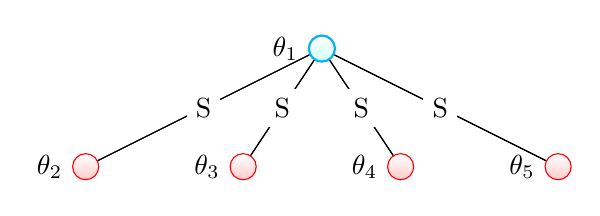
\begin{tikzpicture}[main/.style={c},
		level distance=15mm,
		level 1/.style={sibling distance=20mm},
		level 2/.style={sibling distance=30mm},
		level 3/.style={sibling distance=15mm},
		end/.style = {draw, circle, minimum size=2,fill,top color=white,bottom color=red!20,red},
		discovered/.style = {draw, circle, minimum size=2,fill,color = red}]
		\node (a)[main,label=left:{$\theta_1$}]{}[edge from parent]
		child {
			node (b) [end,label=left:{$\theta_2$}]{}
		}
		child {
			node (c)[end,label=left:{$\theta_3$}]{} 
		}
		child {
			node (d)[end,label=left:{$\theta_4$}]{} 
		}	
		child {
		node (e) [end,label=left:{$\theta_5$}]{} 
		};
		\draw (a) -- (b) node [midway, fill=white] {S};
		\draw (a) -- (c) node [midway, fill=white] {S};
		\draw (a) -- (d) node [midway, fill=white] {S};
		\draw (a) -- (e) node [midway, fill=white] {S};
	\end{tikzpicture}
	\caption{Agent $\theta_1$ shares by sending without checking $(A_{1t}=S)$ the story via broadcast to a group of agents (red).}
	\label{fig:broadcast}
\end{figure}

At each round, we assume that an agent acts and picks one of the actions mentioned in the previous paragraph. This sequential process forms a sub-network $G' \subseteq G$ of the original network $G=(V,E)$. We refer this sub-graph as \textit{sharing sub-network} or \textit{sharing tree}, when we are dealing with tree structures, and this sub-graph is known to the platform. For agent $i$ we assume that the \textit{sharing history} he perceives, namely $H_i$, is the unique path from the originator of the story (source) up to agent $i$. As we see in figure ~\ref{fig:histories}, we have the sharing network in which the red edges indicate the sharing history for agent $k$, with prior belief $\theta_k$, in a path and a tree. The sharing network and history for agent $i$ are the same for a path in contrast with a tree, where we assume that agent $i$ knows that the story is shared only by his predecessors. In our analysis we assume that if agent $i$ receives a story from a agent $j$, he cannot receive the same story from another node $l$. As we see in figure ~\ref{fig:histories}, $\theta_5$ receives the story from $\theta_2$ thus $\theta_3$ will not broadcast the story to $\theta_5 $ again.\footnote{We make a discussion for DAG's in general in a final chapter of this thesis.}

\begin{figure}
	\definecolor {processblue}{cmyk}{0.96,0,0,0}
	\definecolor {processred}{cmyk}{0.96,0,0,0}
	\centering
\begin{subfigure}{1\linewidth}
	\centering	
	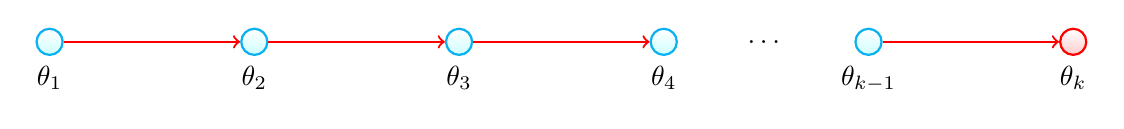
\begin{tikzpicture}[node distance={26mm}, thick, main/.style = {draw, circle, minimum size=2,top color =white , bottom color = processblue!20 ,draw,processblue},end/.style ={draw, circle, minimum size=2,fill,top color=white,bottom color=red!20,red}]
			\node[main,label=below: {$\theta_1$}] (1) {}; 
			\node[main,label=below:{$\theta_2$}] (2) [right of=1] {};
			\node[main,label=below:{$\theta_3$}] (3) [right of=2] {};
			\node[main,label=below:{$\theta_4$}] (4) [right of=3] {};
			\node[main,label=below:{$\theta_{k-1}$}] (5) [right of=4] {};
			\node[end,label=below:{$\theta_k$}] (6) [right of=5] {};
			
			\draw[->,color=red] (1) -- (2);
			\draw[->,color=red] (2) -- (3);
			\draw[->,color=red] (3) -- (4);
			\path (4) -- node[auto=false]{\ldots} (5);
			\draw[->,color=red] (5) -- (6);		
		\end{tikzpicture}
		\subcaption{Sharing path}
\end{subfigure}
\begin{subfigure}{1\linewidth}
	\centering
	\tikzstyle{c} = [thick,draw, circle, minimum size=2,top color =white ,minimum size=2, bottom color = processblue!20,processblue]
		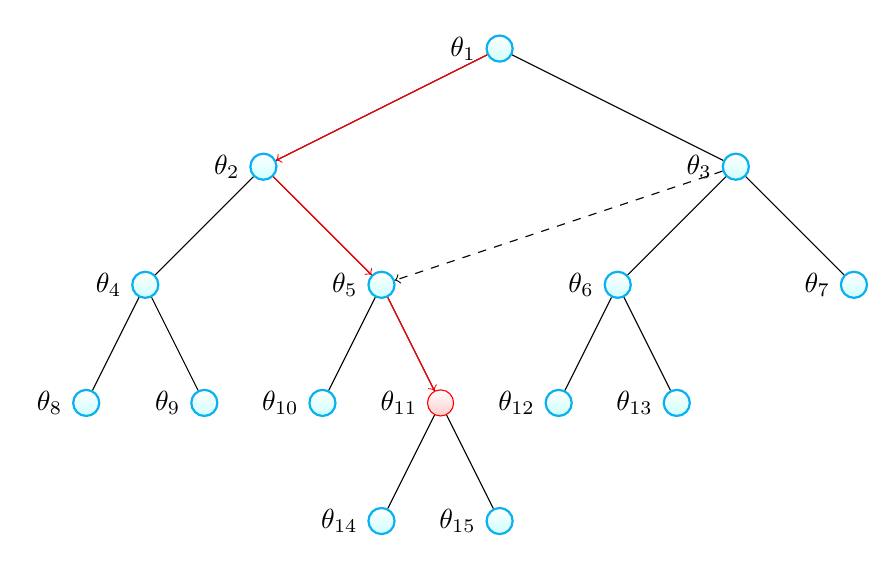
\begin{tikzpicture}[main/.style={c},
			level distance=15mm,
			level 1/.style={sibling distance=60mm},
			level 2/.style={sibling distance=30mm},
			level 3/.style={sibling distance=15mm},
			end/.style = {draw, circle, minimum size=2,fill,top color=white,bottom color=red!20,red},
			discovered/.style = {draw, circle, minimum size=2,fill,color = red}]
			\node (a)[main,label=left:{$\theta_1$}]{}[edge from parent]
			child {
				node (b) [main,label=left:{$\theta_2$}]{}
				child {node [main,label=left:{$\theta_4$}]{}
					child{ node  [main,label=left:{$\theta_8$}]{} }
					child{ node [main,label=left:{$\theta_9$}]{} }
				}
				child {node (c) [main,label=left:{$\theta_5$}]{}
					child{ node [main,label=left:{$\theta_{10}$}]{} }
					child{
						node (d) [end,label=left:{$\theta_{11}$}]{}
						child{ node [main,label=left:{$\theta_{14}$}]{} }
						child{ node [main,label=left:{$\theta_{15}$}]{} }
					}
				}
			}
			child {node (e) [main,label=left:{$\theta_3$}]{} 
				child {node [main,label=left:{$\theta_6$}]{}
					child{ node [main,label=left:{$\theta_{12}$}]{} }
					child{ node [main,label=left:{$\theta_{13}$}]{} }
				}
				child {node [main,label=left:{$\theta_7$}]{}
				}		
			};
			\draw [->,color=red] (a) -- (b);
			\draw [->,color=red] (b) -- (c);
			\draw [->,color=red] (c) -- (d);
			\draw [->,dashed] (e) -- (c);
		\end{tikzpicture}
		\subcaption{Sharing Tree}
\end{subfigure}
		\caption{Sharing process of a story in different structures (a) Path and (b) Binary tree.}
		\label{fig:histories}
\end{figure}

Throughout the process, agents form and update their beliefs about the validity of the story that is being shared in the network, and their validity. There are two basic probabilities that express the agents opinions. First, we have the agents' own posterior belief over the value of ground-truth as well the agents' posterior belief that an article is fake, respectively: 
\begin{equation}\label{eq:beliefs}
	\begin{split}
		b_{it} = P_i \{ \Theta = Y | m = y , H_i \} \\
		q_{it} = P_i \{ V=F | m = y , H_i \}
	\end{split}
\end{equation}
where he receives a message $m=y$ with a history path $H_i$, $\forall t \geq 0$. At each given round $t$ agent updates his own posterior beliefs based on a group of parameters that is common knowledge. The parameters that each agents knows at the round $t$, when he receives the story are:

\begin{itemize}
	\item The sharing history $H_i$ up to him from the source.
	\item His own prior belief $\theta_i$ for the ground-truth.
	\item The ratio of fake news and truthful news that circulate in the platform annotated as $v$.
	\item The credibility $a$ of a true story delivering a correct message about the ground-truth value. 
	\item The probability $\beta$ that a fake story promotes the stance $m=y$ for the  ground-truth variable, irrespectively of its actual value.   
\end{itemize}
With the list of above parameters we calculate the closed form equations for ~\ref{eq:beliefs} that are the posterior beliefs of an agent $i$.
\begin{prop}
	For each $i$ agent at each round $t \geq 0$ it holds that:
	$$b_{it} = \mathbb{P}_i \{ \Theta = Y | m = y , H_i \} =  \frac{\theta_i[\beta v w_{it}+a(1-v)]}{\beta v w_{it} + [a \theta_i + (1-a)(1-\theta_i)](1-v)}$$
	$$q_{it} = \mathbb{P}_i \{ V=F | m = y , H_i \} = \frac{\beta v w_{it}}{\beta v w_{it} + [a \theta_i + (1-a)(1-\theta_i)](1-v)}$$
where $w_{it} = \displaystyle\prod_{k=0}^{t-1} \frac{S_{ik}}{S_{ik}+C_{ik}}$ and $w_{i0} = 1$
\label{prop:beliefs}
\end{prop}

\begin{proof}
We construct the equation for $q_{it}$ since it is the main quantity that we will consider mostly in our work and the proof for $b_{it}$ is equivalent. 
The beliefs of this model are defined over the set $G =\{(\Theta , V )\}_{\Theta \in \{Y,N\},V \in \{T,F\}}$ and according to our model for fake news and the independence of $V$ and $\Theta$, we have the prior opinions of an agent as:
	\begin{itemize}
		\item $\mathbb{P}_{i0} \{(Y,T)\} = \theta_i (1-v) $
		\item $\mathbb{P}_{i0} \{(Y,F)\} = \theta_i v $
		\item $\mathbb{P}_{i0} \{(N,T)\} = (1-\theta_i) (1-v) $
		\item $\mathbb{P}_{i0} \{(N,F)\} = (1-\theta_i) v $
	\end{itemize}
Suppose an agent $i$ receives a story in round $t$, he uses all the information available to him in order to form his posterior belief that a story is fake. The only quantity that changes as time passes is $H_i$. For an opinion $g \in G$ we have the agents' posterior belief:
\begin{equation}
	\begin{split}
		\mathbb{P}_{it} \{g \mid m=y , H_i\} = \frac{\mathbb{P}_{} \{m=y , H_i \mid g\}\mathbb{P}_{} (g)}{\displaystyle\sum_{g' \in G}^{}\mathbb{P}_{} \{m=y , H_i \mid g'\}\mathbb{P}_{} (g')} = 
		\\ =\frac{\mathbb{P}_{} \{ H_i \mid m=y , g\} \mathbb{P}_{} \{ m=y \mid  g\} \mathbb{P}_{} (g)}{\displaystyle\sum_{g' \in G}^{}\mathbb{P}_{} \{ H_i \mid m=y , g'\} \mathbb{P}_{} \{ m=y \mid  g'\} \mathbb{P}_{} (g')}
	\end{split}
\end{equation}
which is the generalized Bayesian inference of an opinion $g$ among a set of opinions $G$. Now we calculate each probability in that expression in order to form $q_{it}$. From section ~\ref{sec:FKNews param} we have the probabilities below:
$$\mathbb{P}_{} \{ m=y \mid (Y,T)\} = a, \mathbb{P}_{} \{ m=y \mid (N,T)\} = 1-a,$$
$$ \mathbb{P}_{} \{ m=y \mid (N,F)\} = \mathbb{P}_{} \{ m=y \mid (Y,F)\} = \beta$$
Now we calculate the quantity $\mathbb{P}_{} \{ H_i \mid m=y , g\}$ which is the probability of a history given a $m=y$ story and an opinion. We are given that the story is $y$, thus agent $i$ considers his strategy only on $V$. This means that a fake story is shared only by action $S$ and a truthful story either by $S$ or $C$:
$$\mathbb{P}_{} \{ H_i \mid m=y , (Y,F)\} = \mathbb{P}_{} \{ H_i \mid m=y , (N,F)\} = $$ $$ \displaystyle\prod_{k=0}^{t-1}\mathbb{P}_{} \{ A_{it}=S \mid m=y , H_i\} =S_{it}$$ 
and
$$\mathbb{P}_{} \{ H_i \mid m=y , (Y,T)\} = \mathbb{P}_{} \{ H_i \mid m=y , (N,T)\} = $$ $$ =\displaystyle\prod_{k=0}^{t-1} [\mathbb{P}_{} \{ A_{it}=S \mid m=y , H_i\} + \mathbb{P}_{} \{ A_{it}=C \mid m=y , H_i\} ]= S_{it} +C_{it}$$
Combining all the above equations, we can compute $q_{it}$:

\begin{align*}
	\begin{split}
		q_{it} & = \mathbb{P}_{it} \{g \mid m=y , H_i\} = \mathbb{P}_{it} \{(Y,F) \lor (N,F) \mid m=y , H_i\} = \\
		& = \frac{\beta v w_{it}}{\beta v w_{it} + [a \theta_{i0}+(1-a)(1-\theta_{i0})](1-v)}
	\end{split}	
\end{align*}
Using the above calculations we can calculate $b_{it}$ in the same way as:

\begin{align*}
	\begin{split}
		b_{it} & = \mathbb{P}_{it} \{g \mid m=y , H_i\} = \mathbb{P}_{it} \{(Y,T) \lor (Y,F) \mid m=y , H_i\} = \\
		& = \frac{\theta_i[\beta v w_{it}+a(1-v)]}{\beta v w_{it} + [a \theta_i + (1-a)(1-\theta_i)](1-v)}
	\end{split}	
\end{align*}
where $w_{it} = \displaystyle\prod_{k=0}^{t-1} \frac{S_{ik}}{S_{ik}+C_{ik}}$, $w_{i0} = 1$ is the proportion probability that a story creates a sharing tree $G'$ that is made with $A_{it} = S$ up to round $t$ where $S_{ik}$ and $C_{ik}$ are given by definition ~\ref{def:ActionProbabilities}.
 
\end{proof}

Throughout the sharing process, each agent acts only once and he receives the appropriate reward for his action. We define the utility of agent $i$, over his action $A$, the function $U_i(A_{it})$. Agent $i$ receives reward either if he blocks a fake story or chooses to share a truthful story. On the other hand, he receives no reward if he blocks a truthful story or shares a fake story. Finally, an agent that chooses to inspect a story, does so by paying a price. Notice that the above function is evaluated only for the variables $V$ and $A_{it}$. Collectively, the induced evaluation function is the following:

\begin{equation}
U_i(A_{it}) = 
\begin{cases}
	1, & (A_{it} = S \land V=T) \lor (A_{ih} = B \land V=F) \\
	0, & (A_{it} = B \land V=T) \lor (A_{ih} = S \land V=F) \\
	1-K, & A_{it} = C \\
\end{cases} 
\end{equation}
where $K$ is the cost of inspection. We assume that inspection occurs with a cost $K < 0.5$ to avoid trivial cases where inspection is never optimal strategy. Agents are choosing actions that maximize their utility at $t$-round and in order to do so, they rely on their beliefs for values about the ground truth that we defined in proposition ~\ref{prop:beliefs}. Each agent chooses the strategy that maximizes his expected utility, given his belief that the story is fake, $q_{it}$. The expected utility can be calculated with the next proposition: 

\begin{prop}
	The expected utility of agents action is given by the function:
	$$\mathbb{E} [U_i(A_{ih})] = 
	\begin{cases}
		1-q_{ih}, & A_{ih} = S  \\
		q_{ih}, & A_{ih} = B  \\
		1-K, & A_{ih} = C \\
	\end{cases} $$
	\label{prop:ExpUtility}
\end{prop}

\begin{proof}
	And agent receives reward if he shares truthful stories or blocks fake according to his belief. Thus, agents $j$ expectation for action send, according to his belief $q_{jt}$  in round $t$, is $\mathbb{E} [U_j(S)] =  (1-q_{jt}) U_j (S \land T) + q_{jt} U_j (S \land F)=1-q_{jt}$. In similar manner we have that expected utility gained from blocking a story, based on agents $j$ belief that is fake, is $\mathbb{E} [U_j(S)] =  (1-q_{jt}) U_j (B \land T) + q_{jt} U_j (B \land F)=q_{jt}$. Finally, if a rational agent chooses to inspect a story based on his updated belief, the expected utility can be calculated as $\mathbb{E} [U_j(C)] =  (1-q_{jt}) U_j (S \land T) + q_{jt} U_j (B \land F)-K=1-q_{jt}+q_{jt}-K=1-K$ where the subtraction of $K$ presents the cost that agent $j$ pays in order to inspect a story and decide whether to send a truthful story or block it otherwise.
\end{proof}

In figure ~\ref{fig:utilities} we have an illustration of the utility curves over different values of $\theta_i$. Figure ~\ref{fig:utilities} is also a visual justification for the assumption that we made for $K < 0.5$. We can clearly see that if we assigned a value greater than $0.5$, then $1-K<0.5$ which implies that $U_i(B) > U_i(C)$, $\forall \theta_i \in (0,\overline{\theta})$ where $U_i(B)$ and $U_i(S)$ intersect, and after that point it holds that $U_i(S) > U_i(C)$,  $\forall \theta_i \in (\mu,1)$.

\begin{figure}[t]
\centering
\includegraphics[width=.75\textwidth]{Figures/utilities.png}
%\includegraphics[width=.75\textwidth, height=.3\textheight]{Figures/line_plot.pdf}

\caption{The expected utility curves over different prior beliefs that follow a Gaussian distribution at first round. Parameters: $v=K=0.4$, $a=90\%$ and $\theta_i \sim \mathcal{N} (\mu=0.3,\sigma^2=0.09)$.}

\label{fig:utilities}
\end{figure}

\section{Propagation Dynamics}
\label{ch:Dynamics}

In this section we will focus on the dynamics of agents propagation and the properties of our setup, in order to help us tackle the main problem which is the optimal time that we can intervene to stop the propagation of a fake story. In order to introduce the properties, we describe each individual step of the process in a sharing tree. The proofs for theorems, propositions and lemmas that are mentioned in related work are provided in ~\ref{app:AppendixA}.

At each round $t$ an agent $i$ is up to decide if he will inspect a story $m=y$ and then if he will share it via a broadcast on a group of agents, i.e. his followers.\footnote{The choice of agents that are going to react and how it affects the sharing tree and the inspection time is further studied later on this thesis.} According to his belief, he evaluates each strategy and picks the one with that maximizes his expected utility. If he decides to share the story, he broadcasts the story to the set of all its out-neighbors (i.e., his$\backslash$her followers) in the underlying social-network graph. In round $t+1$, we pick another agent to act in a sense that round $t$ is a counter that determines how many agents have reacted. On the other hand, if an agent $j$ decides to not share the story, no matter if he inspects or not, the sharing history $H_j$ is discontinued at his path. Notice that in case of paths, time and agents are equivalent in the sense that we can refer to each agent as $t$ agent that is up to act. Additionally, if an agent decides not to share the story, the whole process is discontinued while in an $m$-ary tree it stops only in the particular sub-tree whose root node decides not to share. 

\begin{figure}
	\definecolor {processblue}{cmyk}{0.96,0,0,0}
	\definecolor {processred}{cmyk}{0.96,0,0,0}
	\tikzstyle{c} = [thick,draw, circle, minimum size=2,top color =white ,minimum size=2, bottom color = processblue!20,processblue]
	\begin{minipage}{.3\textwidth}
		\subcaption{}
		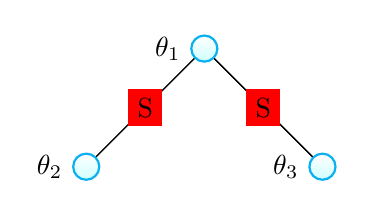
\begin{tikzpicture}[main/.style={c},
			level distance=15mm,
			level 1/.style={sibling distance=30mm},
			level 2/.style={sibling distance=20mm},
			level 3/.style={sibling distance=10mm},
			end/.style = {draw, circle, minimum size=2,fill,top color=white,bottom color=red!20,red},
			discovered/.style = {draw, circle, minimum size=2,fill,color = red}]
			\node (1)[main,label=left:{$\theta_1$}]{}[edge from parent]
			child {
				node (2) [main,label=left:{$\theta_2$}]{}
			}
			child {
				node (3)[main,label=left:{$\theta_3$}]{} 
			};
			
			\draw (1) -- (2) node [midway, fill=red] {S};
			\draw (1) -- (3) node [midway, fill=red] {S};
		\end{tikzpicture}
		
	\end{minipage}
	\begin{minipage}{.3\textwidth}
		\subcaption{}
		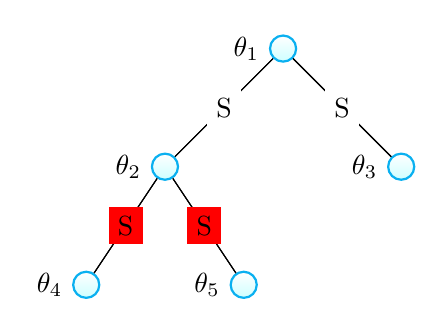
\begin{tikzpicture}[main/.style={c},
			level distance=15mm,
			level 1/.style={sibling distance=30mm},
			level 2/.style={sibling distance=20mm},
			level 3/.style={sibling distance=10mm},
			end/.style = {draw, circle, minimum size=2,fill,top color=white,bottom color=red!20,red},
			discovered/.style = {draw, circle, minimum size=2,fill,color = red}]
			\node (1)[main,label=left:{$\theta_1$}]{}[edge from parent]
			child {
				node (2) [main,label=left:{$\theta_2$}]{}
				child {
					node (4) [main,label=left:{$\theta_4$}]{}
				}
				child {
					node (5)[main,label=left:{$\theta_5$}]{}
				}
			}
			child {
				node (3)[main,label=left:{$\theta_3$}]{} 
			};
			\draw (1) -- (2) node [midway, fill=white] {S};
			\draw (1) -- (3) node [midway, fill=white] {S};
			\draw (2) -- (4) node [midway, fill=red] {S};
			\draw (2) -- (5) node [midway, fill=red] {S};
		\end{tikzpicture}
		
	\end{minipage}
	\begin{minipage}{.3\textwidth}
		\subcaption{}
		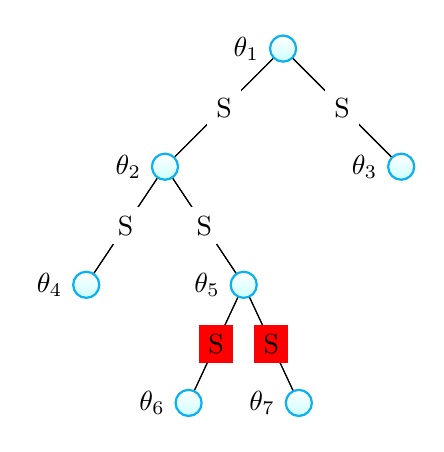
\begin{tikzpicture}[main/.style={c},
			level distance=15mm,
			level 1/.style={sibling distance=30mm},
			level 2/.style={sibling distance=20mm},
			level 3/.style={sibling distance=14mm},
			end/.style = {draw, circle, minimum size=2,fill,top color=white,bottom color=red!20,red},
			discovered/.style = {draw, circle, minimum size=2,fill,color = red}]
			\node (1)[main,label=left:{$\theta_1$}]{}[edge from parent]
			child {
				node (2) [main,label=left:{$\theta_2$}]{}
				child {
					node (4) [main,label=left:{$\theta_4$}]{}
				}
				child {
					node (5)[main,label=left:{$\theta_5$}]{}
					child {node (6)[main,label=left:{$\theta_6$}]{}}
					child {node (7)[main,label=left:{$\theta_7$}]{}}
				}
			}
			child {
				node (3)[main,label=left:{$\theta_3$}]{} 
			};
			
			\draw (1) -- (2) node [midway, fill=white] {S};
			\draw (1) -- (3) node [midway, fill=white] {S};
			\draw (2) -- (4) node [midway, fill=white] {S};
			\draw (2) -- (5) node [midway, fill=white] {S};
			\draw (5) -- (6) node [midway, fill=red] {S};
			\draw (5) -- (7) node [midway, fill=red] {S};
		\end{tikzpicture}
		
	\end{minipage}
	\begin{minipage}{.5\textwidth}
		\subcaption{}
		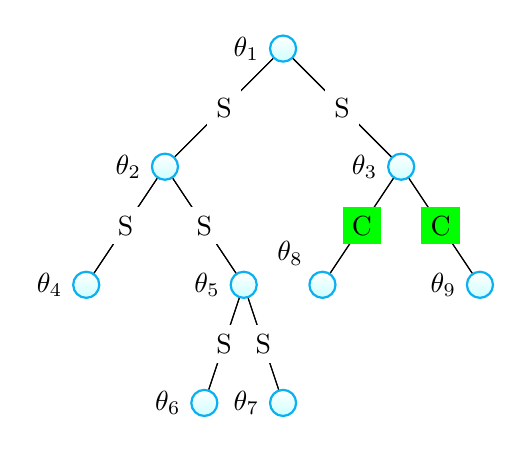
\begin{tikzpicture}[main/.style={c},
			level distance=15mm,
			level 1/.style={sibling distance=30mm},
			level 2/.style={sibling distance=20mm},
			level 3/.style={sibling distance=10mm},
			end/.style = {draw, circle, minimum size=2,fill,top color=white,bottom color=red!20,red},
			discovered/.style = {draw, circle, minimum size=2,fill,color = red}]
			\node (1)[main,label=left:{$\theta_1$}]{}[edge from parent]
			child {
				node (2) [main,label=left:{$\theta_2$}]{}
				child {
					node (4)[main,label=left:{$\theta_4$}]{}
				}
				child {
					node (5)[main,label=left:{$\theta_5$}]{}
					child {node (6)[main,label=left:{$\theta_6$}]{}}
					child {node (7)[main,label=left:{$\theta_7$}]{}}
				}
			}
			child {
				node (3)[main,label=left:{$\theta_3$}]{}
				child {node (8)[main,label=above left:{$\theta_8$}]{}}
				child {node (9)[main,label=left:{$\theta_9$}]{}}
			};
			
			\draw (1) -- (2) node [midway, fill=white] {S};
			\draw (1) -- (3) node [midway, fill=white] {S};
			\draw (2) -- (4) node [midway, fill=white] {S};
			\draw (2) -- (5) node [midway, fill=white] {S};
			\draw (5) -- (6) node [midway, fill=white] {S};
			\draw (5) -- (7) node [midway, fill=white] {S};
			\draw (3) -- (8) node [midway, fill=green] {C};
			\draw (3) -- (9) node [midway, fill=green] {C};
		\end{tikzpicture}
		
	\end{minipage}
	\begin{minipage}{.5\textwidth}
		\centering
		\subcaption{}
		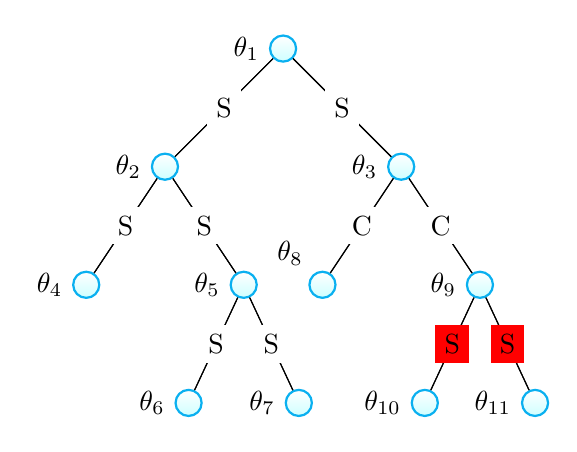
\begin{tikzpicture}[main/.style={c},
			level distance=15mm,
			level 1/.style={sibling distance=30mm},
			level 2/.style={sibling distance=20mm},
			level 3/.style={sibling distance=14mm},
			end/.style = {draw, circle, minimum size=2,fill,top color=white,bottom color=red!20,red},
			discovered/.style = {draw, circle, minimum size=2,fill,color = red}]
			\node (1)[main,label=left:{$\theta_1$}]{}[edge from parent]
			child {
				node (2) [main,label=left:{$\theta_2$}]{}
				child {
					node (4)[main,label=left:{$\theta_4$}]{}
				}
				child {
					node (5)[main,label=left:{$\theta_5$}]{}
					child {node (6)[main,label=left:{$\theta_6$}]{}}
					child {node (7)[main,label=left:{$\theta_7$}]{}}
				}
			}
			child {
				node (3)[main,label=left:{$\theta_3$}]{}
				child {node (8)[main,label=above left:{$\theta_8$}]{}}
				child {node (9)[main,label=left:{$\theta_9$}]{}
					child {node (10)[main,label=left:{$\theta_{10}$}]{}}
					child {node (11)[main,label=left:{$\theta_{11}$}]{}}
				}
			};
			
			\draw (1) -- (2) node [midway, fill=white] {S};
			\draw (1) -- (3) node [midway, fill=white] {S};
			\draw (2) -- (4) node [midway, fill=white] {S};
			\draw (2) -- (5) node [midway, fill=white] {S};
			\draw (5) -- (6) node [midway, fill=white] {S};
			\draw (5) -- (7) node [midway, fill=white] {S};
			\draw (3) -- (8) node [midway, fill=white] {C};
			\draw (3) -- (9) node [midway, fill=white] {C};
			\draw (9) -- (10) node [midway, fill=red] {S};
			\draw (9) -- (11) node [midway, fill=red] {S};
		\end{tikzpicture}
		
	\end{minipage}
	\caption{The resulting sharing tree after five reactions, from $(a)$ to $(e)$.}
	\label{fig:SharingProcc}
\end{figure}

Before we further continue our study, it is time to illustrate each individual step of a sharing process with an extended example. Using figure ~\ref{fig:SharingProcc}, we begin with agent $1$ with $\theta_1$ that chooses to share the story $m=y$ with his neighbors. In order to do that, evaluates his expected utility for each action and picks the appropriate that has the maximum value. In order to do so, he calculates his posterior belief. In the beginning of the process, there is no sharing history since he is the first that reacts to the story on his unique path from the source up to him (i.e. he is the root). From proposition ~\ref{prop:beliefs} we have that $q_{11}= \displaystyle\frac{\beta v w_{11}}{\beta v w_{11} + [a \theta_{1}+(1-a)(1-\theta_{1})](1-v)}$ where $w_{11}=S_0/(S_0+C_0)$ since there is no previous sharing history. Continuing with the next agent $ \theta_2$ in $(b)$ he also evaluates his own posterior belief with the expected utility and he finds that it maximizes when he chooses to share with out checking as well. The difference this time is that the sharing history of his ancestors is non trivial, thus he has to make an estimation about $w_{it}$. In order to do so, he must calculate $w_{22} = \displaystyle\prod_{k=0}^{1} \frac{S_{ik}}{S_{ik}+C_{ik}}$ which translates to the probability \textit{that a story reaches to agent $i$ without any inspection} and it is a proportion of $q_{it}$. We notice that this quantity demands the knowledge of probabilities that concern the sharing actions of previous agents in his sharing history. It is obvious that if agent $i$ knew the prior beliefs of their ancestors, then agent $i$ would have a best response strategy and the choice of action would be deterministic. Since we want to study a model that works under uncertainty, we introduce the next two assumptions:
\begin{assumption}
Aside for the parameters that we assumed in section ~\ref{sec:SharingProc} is shared throughout all agents and in order for agent to update his belief by calculating $w_{it} = \displaystyle\prod_{k=0}^{t-1} \frac{S_{ik}}{S_{ik}+C_{ik}}$, we have two options:
	\begin{itemize}
		\item Agents presume that all prior opinions follow a normal distribution, $\theta_i \sim \mathcal{N} (\theta^*,\sigma^2)$, and $\theta^*$ is common knowledge in our social network $\forall i$.
		\item Agents presume that all prior opinions follow a normal distribution and each agent creates his own normal distribution centralized around him such that $\theta_j \sim \mathcal{N}_i (\theta^*,\sigma^2)$ with $\theta^* = \theta_i$, $\forall j$.
	\end{itemize}
\label{assum:AgentsPerceptionOfThetas}
\end{assumption}
The first option translates to a setup that agents determine past reactions based on a average prior opinion, i.e. an average value based on a similar subject that platform historically recorded in the social network. This approach creates a normalized sharing behavior because agents are assumed to be completely homogeneous, in the sense that they all sample exactly the same distribution when considering the prior beliefs of other agents. On the other hand, when agent $i$ uses his prior opinion to determine the reaction history up to him, e centers the normal distribution for sampling the other agents' prior beliefs to its own (actual) prior belief. I.e., the agents are now assumed to be heterogeneous.

Continuing in figure ~\ref{fig:SharingProcc}, at $(d)$ and $(e)$ derived sub-trees in our sharing process, we see that agent $\theta_3$ is choosing to inspect the information and share it with his neighbors, $\theta_8$ and $\theta_9$. For our model, and since we assumed that the inspection yields perfect outcome, it is sufficient to find an agent that inspected the story and chose to share it. This observation is useful in the next chapter that is focused on platform's inspection problem and the solution of interrupting probable viral stories that are shared with suspicious reactions.

In order to separate the actual probabilities that an agent $i$ chooses a strategy between $\{B,C,S\}$ from his estimated value about those probabilities for his ancestors, we introduce the next annotations:

\begin{definition}
	We define as $B_{it}^j,C_{it}^j,S_{it}^j$ the probabilities that agent $i$ observes for agent $j$ and his actions $\{B,C,S\}$ respectively for round $t$. More specifically, we have the equations below:
		$$B_{it}^j=\mathbb{P}_{i} \{A_{jt}(\theta_i^*) = B \mid m=y , H_j\}$$
		$$C_{it}^j=\mathbb{P}_{i} \{A_{jt}(\theta_i^*) = C \mid m=y , H_j\}$$
		$$S_{it}^j=\mathbb{P}_{i} \{A_{jt}(\theta_i^*) = S \mid m=y , H_j\}$$
where $A_{jt}(\theta_i^*)$ is the action that agent $i$ believes that is optimal for agent $j$ according to the assumption ~\ref{assum:AgentsPerceptionOfThetas} where agent $i$ presumes that his predecessors acting with some prior $\theta^*$.
\label{def:PresumedActionProbs}
\end{definition}

Now we provide closed form equations for probabilities in definitions ~\ref{def:ActionProbabilities} and ~\ref{def:PresumedActionProbs}, derived from the above proposition.
\begin{prop}
	Let be agent $i$ that is up to react in round $t$. Then for the probabilities $B_{it},C_{it},S_{it}$ it holds that:
	$$B_{it} = \mathcal{F} \left( \displaystyle\frac{1}{2\alpha-1}\left[\frac{\beta v w_{it} K}{(1-v)(1-K)}-(1-\alpha)\right] \right)$$

	$$S_{it} = 1-\mathcal{F} \left( \displaystyle\frac{1}{2\alpha-1}\left[\frac{\beta v w_{it} (1-K)}{(1-v)K}-(1-\alpha)\right] \right)$$  
	
	$$C_{it} = 1-B_{it}-S_{it}$$
where $\mathcal{F}$ is the cumulative distribution function (cdf) from where $\theta_i$'s are drawn. 
\label{prop:CloseProbabilitiesActions}
\end{prop}

It is important to notice that in proposition ~\ref{prop:CloseProbabilitiesActions}, the formulation is independent of the cdf $\mathcal{F}$ that distribution has. In our model we assumed that tall the agents, and the platform, presume that the other agents' prior beliefs are drawn independently from a normal distribution $N(\mu,\sigma^2)$

$$\mathcal{F}(x) = \frac{1}{2} \left[1+erf\left(\frac{x-\mu}{\sigma \sqrt{2}}\right)\right]$$
where $erf(x)$ is the error function specified in the background.

Now that we have the appropriate tools and specified the all the assumptions about how an agent processes information and how he acts, we are ready to analyze each component of our setup and find useful properties that will help us tackle the platform's inspection problem. One important property that will help in the analysis of this model is the monotonicity of $q_{it}$. The following lemmas from ~\cite{papanastasiou} are useful tools throughout the analysis.

\begin{lemma}
	Suppose that an agent receives a story in round $t$. The agent's posterior belief that the story is fake, $q_{it}$, is strictly decreasing in her prior opinion over ground truth, $\theta_i$.
	\label{lemma:prior}
\end{lemma}
\begin{lemma}
	Suppose that an agent receives a story in round $t$ with a sharing history $H_i$ and a prior belief over $\Theta$, $\theta_i$. The agent's posterior belief that this story is fake is decreasing as $t$ increases.
	\label{lemma:monotontime} 
\end{lemma}
The probability $q_{it}$ can be seen as a sequence of $\theta_i$, $\{q_{it}\}_{\theta_i \sim \mathcal{N} (\mu, \sigma)}$ for fixed $t$'s, or as a sequence of $t$, $\{q_{it}\}_{t \in \mathbb{N}}$ by fixing agents to their prior opinions.  Lemma ~\ref{lemma:prior} describes the behavior of $q_{it}$ as we adjust the prior opinion of an agent, while \ref{lemma:monotontime} expresses the monotonicity of $q_{it}$ as time approaches to infinity. From ~\ref{lemma:prior} we notice that for a given round $t_0$, if agents' prior belief that $\Theta = Y$ is closer to 1 then it is less likely that he will perceive that the story is fake. In addition, in lemma \ref{lemma:monotontime} we see that the later an agent receives a story he is less likely to believe that it is fake. In other words, as the length of $H_i$ increases\footnote{We remind that the sharing history $H_i$ is a path from the root to a node in a sharing tree $G' \subseteq G$.} up to an agent $i$, he is more willing to believe that some agent $j$, between the originator of the story up to him, has inspected the story and found its content truthful. Lemmas ~\ref{lemma:prior} and ~\ref{lemma:monotontime} are very important to extract properties for the behavior of agents as well for the optimal solution for the platform that we will analyze in the next chapter. 



As soon as an agent receives a story and based on ~\ref{prop:ExpUtility}, his best response is the one that maximizes his expected utility thus, every action $A_{it}$ occurs with probability that depends on his belief that a story is fake $q_{it}$. Using definition ~\ref{def:ActionProbabilities} for those probabilities combined the above proposition we derive bounds of our sharing process.

\begin{prop}
	In any round $t$, there exists a lower and an upper bound $\underline{Z}_{it}, \overline{Z}_{it} \in [0,1]$ respectively, for agent $i$, such that:
	
	\begin{enumerate}
		\item If $\theta_i < \underline{Z}_{it}$ then $A_{it}=B$.
		\item If $\theta_i > \overline{Z}_{it}$ then $A_{it}=S$.
		\item If $\underline{Z}_{it} \leq \theta_i \leq \overline{Z}_{it}$ then $A_{it}=C$.
	\end{enumerate}
where the thresholds $\underline{Z}_{it}$ and  $\overline{Z}_{it}$ expressed as:
$$\underline{Z}_{it}=\displaystyle\frac{1}{2\alpha-1}\left[\frac{\beta v w_{it} K}{(1-v)(1-K)}-(1-\alpha)\right]$$
$$\overline{Z}_{it}=\displaystyle\frac{1}{2\alpha-1}\left[\frac{\beta v w_{it} (1-K)}{(1-v)K}-(1-\alpha)\right]$$
	\label{prop:ZBounds}
\end{prop}

Proposition ~\ref{prop:ZBounds} shows that at any given time, the optimal choice of strategy that maximizes the expected utility of an agent is bounded within the above thresholds $\underline{Z}_{it}$and $ \overline{Z}_{it}$. Notice that we can slightly modify proposition ~\ref{prop:ZBounds} in a way such that they become sequences over $\theta_i$ for a given round $t$. This brings us to the next corollary: 

\begin{corollary}
	For all agents $i$, there exists thresholds with $\theta_i$ as argument such that:
	$$ \overline{W}_{i}=\frac{1-K}{K}\frac{1-v}{v}\frac{2\alpha-1}{\beta}\left(\theta_i+\frac{1-a}{2\alpha-1}\right) < w_{it} $$
	$$ \underline{W}_{i}=\frac{K}{1-K}\frac{1-v}{v}\frac{2\alpha-1}{\beta}\left(\theta_i+\frac{1-a}{2\alpha-1}\right) > w_{it} $$
	equivalent to $\underline{Z}_{it} \overline{Z}_{it} \in [0,1]$ respectively.
	\label{cor:AlternativeBounds}
\end{corollary}
The last corollary is an alternative expression of thresholds $\underline{Z}_{it}$ and $\overline{Z}_{it}$ with the advantage that they are not dependent on time $t$. With the help of corollary ~\ref{cor:AlternativeBounds}, instead monitoring the sliding window where it is formed from $\underline{Z}_{it\rightarrow \infty}, \overline{Z}_{it\rightarrow \infty}$, we can calculate the round $t$ where $w_{it_0}$ escapes out of $\underline{W}_{i}$, $ \overline{W}_{i} \in [0,1]$  thresholds. We remind that $w_{it}$ is a proportion of the actual belief, for agent $i$, that the story is fake. The sequence $w_{it} \propto q_{it}$ calculates the amount of shares that made without inspection in the process, namely $A_{it}=S$. Corollary ~\ref{cor:AlternativeBounds} is very useful for platforms mechanism in order to answer which stories are probably fake based on the propagation and we further exploit their properties in chapter ~\ref{ch:Platforms Problem}.

\begin{figure}[t]
	\centering
	\includegraphics[width=.75\textwidth]{Figures/Zbounds.pdf}
	%\includegraphics[width=.75\textwidth, height=.3\textheight]{Figures/Zbounds.pdf}
	
	\caption{Regions (areas according to high and low thresholds) that characterize agents actions for different prior opinions in first round. Parameters: $v=K=0.4$, $a=90\%$ and $\theta_i \sim \mathcal{N} (\mu=0.3,\sigma^2=0.09)$.}
	
	\label{fig:boundsandAreas}
\end{figure}

In figure ~\ref{fig:boundsandAreas}, we have a Gaussian pdf and the bounds $\underline{Z}, \overline{Z}$ in first round $t=0$. We have three cases where:

\begin{itemize}
	\item Priors $\theta_i$ that are picked below $\underline{Z}$, inside the red area, consists of users that prefer to block the sharing process without even inspecting it.
	\item The green area, that is between the thresholds $\underline{Z}, \overline{Z}$, consists of agents with prior opinions such that they are more likely to check the story in first round.
	\item The blue area, above $\overline{Z}$ threshold, belongs to agents with such prior opinions that they are going to share the message with no inspection.
\end{itemize}

Now we proceed, with the next proposition, by proving that those thresholds are non increasing in $t$ and also the difference $|\overline{Z}_{it} - \underline{Z}_{it}|$ is non increasing and non zero while $t \rightarrow \infty$.

\begin{prop}
	Given an agent $j$ and thresholds $\underline{Z}_{jt}$, $ \overline{Z}_{jt} \in (0,1)$, it holds that $\underline{Z}_{jt}$ and $ \overline{Z}_{jt}$ are decreasing in $t$ as well as the difference  $|\overline{Z}_{jt} - \underline{Z}_{jt}|_{t \rightarrow \infty}$
	\label{prop:decreasingZetas}
\end{prop}

\begin{proof}
	The claim is complete if we prove that $w_{it}$ is non increasing. That is obvious since $w_{it} = \displaystyle\prod_{k=0}^{t-1} \frac{S_{ik}}{S_{ik}+C_{ik}}$ is an product of quantities such that $ S_{it}, C_{it} \in (0,1)$, thus $w_{jt+1} < w_{jt}$, $\forall t$. For the difference $|\overline{Z}_{it} - \underline{Z}_{it}|$ let's assume that we have a agent $j$ with $\theta_j$, we compare the difference in round $t$ with the next round $t+1$. We have that:
	$$|\overline{Z}_{j(t+1)} - \underline{Z}_{j(t+1)}|-|\overline{Z}_{jt} - \underline{Z}_{jt}|=$$
	
	$$=
	\displaystyle\frac{1}{2\alpha-1}\left[\frac{\beta v w_{j(t+1)} (1-K)}{(1-v)K}-(1-\alpha)\right]-\displaystyle\frac{1}{2\alpha-1}\left[\frac{\beta v w_{j(t+1)} K}{(1-v)(1-K)}-(1-\alpha)\right]- $$
	
	$$\left\{
	\displaystyle\frac{1}{2\alpha-1}\left[\frac{\beta v w_{jt} (1-K)}{(1-v)K}-(1-\alpha)\right]-\displaystyle\frac{1}{2\alpha-1}\left[\frac{\beta v w_{jt} K}{(1-v)(1-K)}-(1-\alpha)\right]\right\}=$$
	
	$$\displaystyle\frac{1}{2\alpha-1} \left[ \frac{\beta v (1-K)}{(1-v)K} (w_{j(t+1)}-w_{jt}) -
	 \frac{\beta v K}{(1-v)(1-K)} (w_{j(t+1)}-w_{jt})\right]=
	$$
	
	$$ = \delta (w_{j(t+1)}-w_{jt})
	$$
	where $\delta$ is a constant such that $\delta>0$ for $K<0.5$ and $a>0.5$. Since $w_{j(t+1)}<w_{jt}$ we have that the difference is decreasing and it is non zero.
	
	The proof is equivalent using the assumption ~\ref{assum:AgentsPerceptionOfThetas} where $S_{it}$ and $C_{it}$ are replaced by $S_{it}^j$ and $C_{it}^j$ respectively, $\forall j \in path(root,i)$.
\end{proof}

With proposition ~\ref{prop:decreasingZetas}, we have the next important corollary for the sharing process, that expands the cascading behavior in ~\cite{papanastasiou} for sharing trees.

\begin{corollary}
	Let $G'$ be a sharing tree as specified in section ~\ref{sec:SharingProc}. There exists a certain depth $h_c$ at which the best response is to share without inspect. More specifically, there is a depth $h_c$ such that $\overline{Z}_{ih_c} \leq 0$ for some agent $i$ or equivalent, $h_c = min \left\{h \mid S_{ih}=1 \text{ or } \overline{Z}_{ih_c} \leq 0\right\}$.
\end{corollary}

\begin{figure}
	\definecolor {processblue}{cmyk}{0.96,0,0,0}
	\definecolor {processred}{cmyk}{0.96,0,0,0}
	\centering
	\tikzstyle{c} = [thick,draw, circle, minimum size=2,top color =white ,minimum size=2, bottom color = processblue!20,processblue]
	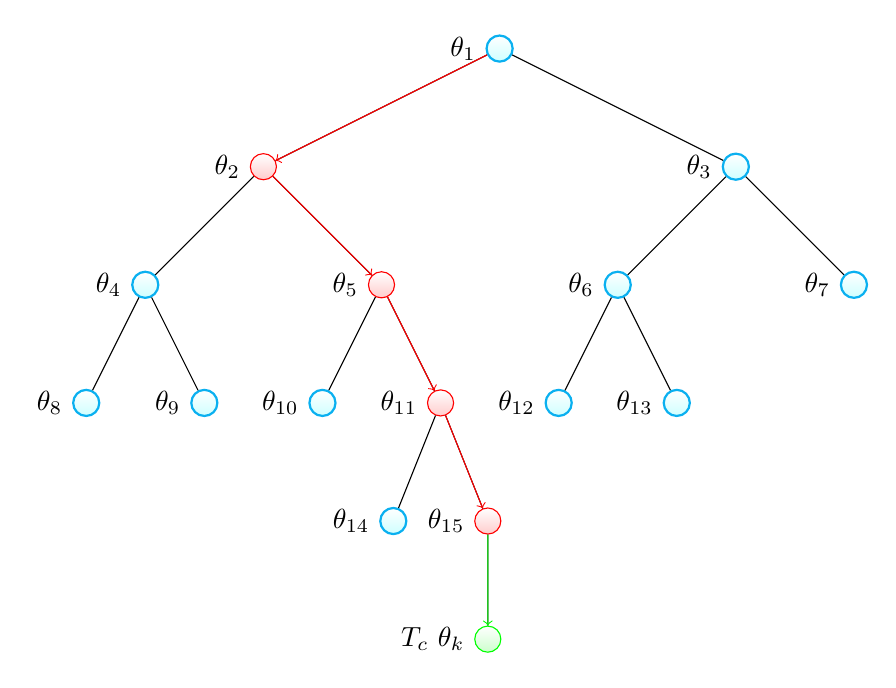
\begin{tikzpicture}[main/.style={c},
		level distance=15mm,
		level 1/.style={sibling distance=60mm},
		level 2/.style={sibling distance=30mm},
		level 3/.style={sibling distance=15mm},
		level 4/.style={sibling distance=12mm},
		end/.style = {draw, circle, minimum size=2,fill,top color=white,bottom color=red!20,red},
		critical/.style = {draw, circle, minimum size=2,fill,top color=white,bottom color=green!20,green}]
		\node (a)[main,label=left:{$\theta_1$}]{}[edge from parent]
		child {
			node (b) [end,label=left:{$\theta_2$}]{}
			child {node [main,label=left:{$\theta_4$}]{}
				child{ node  [main,label=left:{$\theta_8$}]{} }
				child{ node [main,label=left:{$\theta_9$}]{} }
			}
			child {node (c) [end,label=left:{$\theta_5$}]{}
				child{ node [main,label=left:{$\theta_{10}$}]{} }
				child{ node (d) [end,label=left:{$\theta_{11}$}]{}
						child{ node [main,label=left:{$\theta_{14}$}]{} }
						child{ node (k) [end,label=left:{$\theta_{15}$}]{} 
							child{ node (T) [critical,label=left:{$T_c$  $\theta_k$}] {} }
						}
				}
			}
		}
		child {node (e) [main,label=left:{$\theta_3$}]{} 
			child {node [main,label=left:{$\theta_6$}]{}
				child{ node [main,label=left:{$\theta_{12}$}]{} }
				child{ node [main,label=left:{$\theta_{13}$}]{} }
			}
			child {node [main,label=left:{$\theta_7$}]{}
			}		
		};
		\draw [->,color=red] (a) -- (b);
		\draw [->,color=red] (b) -- (c);
		\draw [->,color=red] (c) -- (d);
		\draw [->,color=red] (d) -- (k);
		\draw [->,color=green] (k) -- (T);
	\end{tikzpicture}
\caption{The critical round $T_c$ at where the best response of an agent in that depth is to share without inspecting an event.}
\label{fig:CriticalTime}
\end{figure}

Since each path expands as an independent experiment (agents know only how many of their predecessors shared), for each of these paths there is a certain depth that is critical. In the case of a path, where agents react in sequential manner, the round represents the number of agents that react. In other words, we have a critical agent positioned in a specific spot of the path such that, after a certain amount of reactions, at round $T_c$ the best response of $T_c + 1$ agent is to send without inspecting the story. In figure ~\ref{fig:CriticalTime} we have an example of a sharing process alongside with the propagation network. The sequence of agents $\left\{ \theta_1, \theta_2, \theta_5, \theta_{11}, \theta_15  \right\}$ reached in such depth that the quantity $w_{kT_c}$ will affect agents' belief that the story is fake, $q_{kT_c}$ that the expected response is to share the story without inspection. In other words, agents' interpretation of their depth is an increasing possibility of an existing agent that checked the story and decided to share to the subsequent agents.

One question that emerges from the above analysis is the impact of depth over agents opinion that a story is false, namely $q_{it}$.

\begin{corollary}
	For an agent $i$ with prior opinion $\theta$ and his posterior belief that $m=y$ is fake, $q_{it}$, it holds that:
	\begin{itemize}
		\item If agent $i$ chooses action $S$ in round $t_0$, $A_{it_0} = S$ then $\forall t>t_0$ subsequent rounds, $A_{it}=S$.
		\item If agent $i$ chooses action $B$ in round $t_0$, $A_{it_0} = B$ then $\forall t \in [1,t_0]$ previous rounds, $A_{it}=B$.
	\end{itemize}
	\label{cor:SBBOUNDS}
\end{corollary}

\begin{proof}
	We will prove the first bullet, since the second is proven in symmetrical manner with opposite monotonicity. Lets assume that agent chooses to share a story without inspecting it, at a given time $t_0$ which means that $A_{it_0}=S$. This choice optimal when his expected utility is maximized via action $S$, more specifically, whenever it holds that $1-q_{it_0}>q_{it_0}$ and $1-q_{it_0}>1-K$. Since $q_{it}$ is decreasing in time, then the quantity $1-q_{it_0}$ is increasing in time and since it is upper bound for both $q_{it}$ and $1-K$, then it will remain an upper bound as $t$ increases, which proves the claim. For the second bullet, the proof is symmetric since $q_{it_0}>1-q_{it_0}$ and $q_{it_0}>1-K$ when the response is $A_{it_0}=B$. Adding the fact that $q_{it}$ is decreasing in time, from lemma ~\ref{lemma:monotontime}, we have that the above inequalities hold, for each round $1<t<t_0$.
\end{proof}

